\documentclass[12pt]{article}
\usepackage[landscape]{geometry}
\usepackage{graphicx,color} 
\include{def.tex}


\begin{document}
\pagestyle{empty}

\noindent The flux through a loop is $\phi = 0.1 t^3 + 0.4 t^2$ in webers.  What is the induced EMF as a function of time? 
\newpage

\noindent Consider the configuration below.  The magnitude of the B-field is B, the rod speed is v, and the rods length is l.  What is the induced EMF of the circuit?  If the resistor has resistance of R, what is the force needed to move the rod at constant speed?

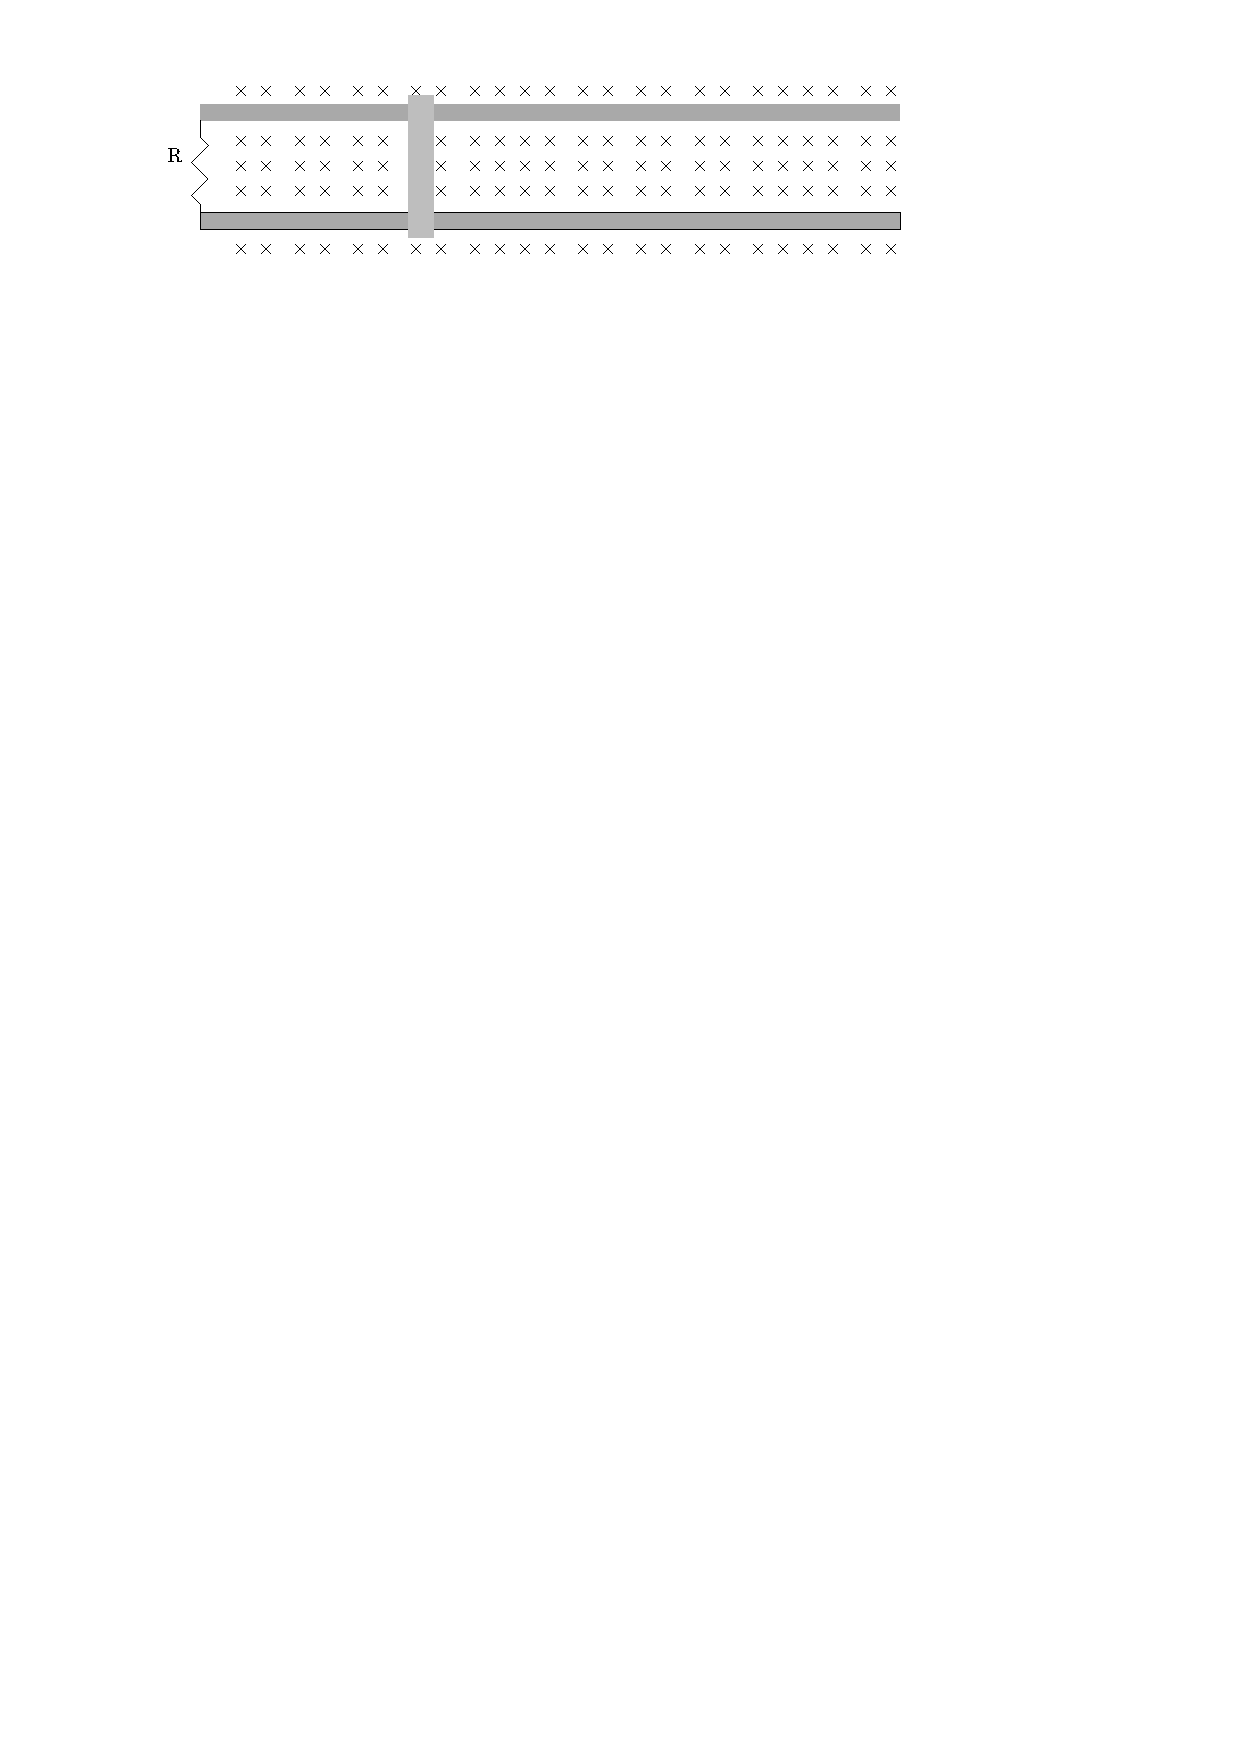
\includegraphics[width=0.7\textwidth]{magnetic_rod.pdf}
\newpage


\noindent Consider a coaxial cable that consists of two thin conducting infinite cylinders with radius $r_1$ and $r_2$ with $r_1 < r_2$.  The currents on the inner and outer are equal in magnitude and opposite in direction.  As an exercise in Ampere's law, find the magnetic flux between the cylinders though a surface that goes from $r_1$ to $r_2$ and length $l$. 

\newpage

\noindent Consider the following circuit.  At t=0, switch S is thrown.  Find the power that flows through the resistor as a function of $t$.  At what time is the power half of what the power would be at $t=\infty$ 

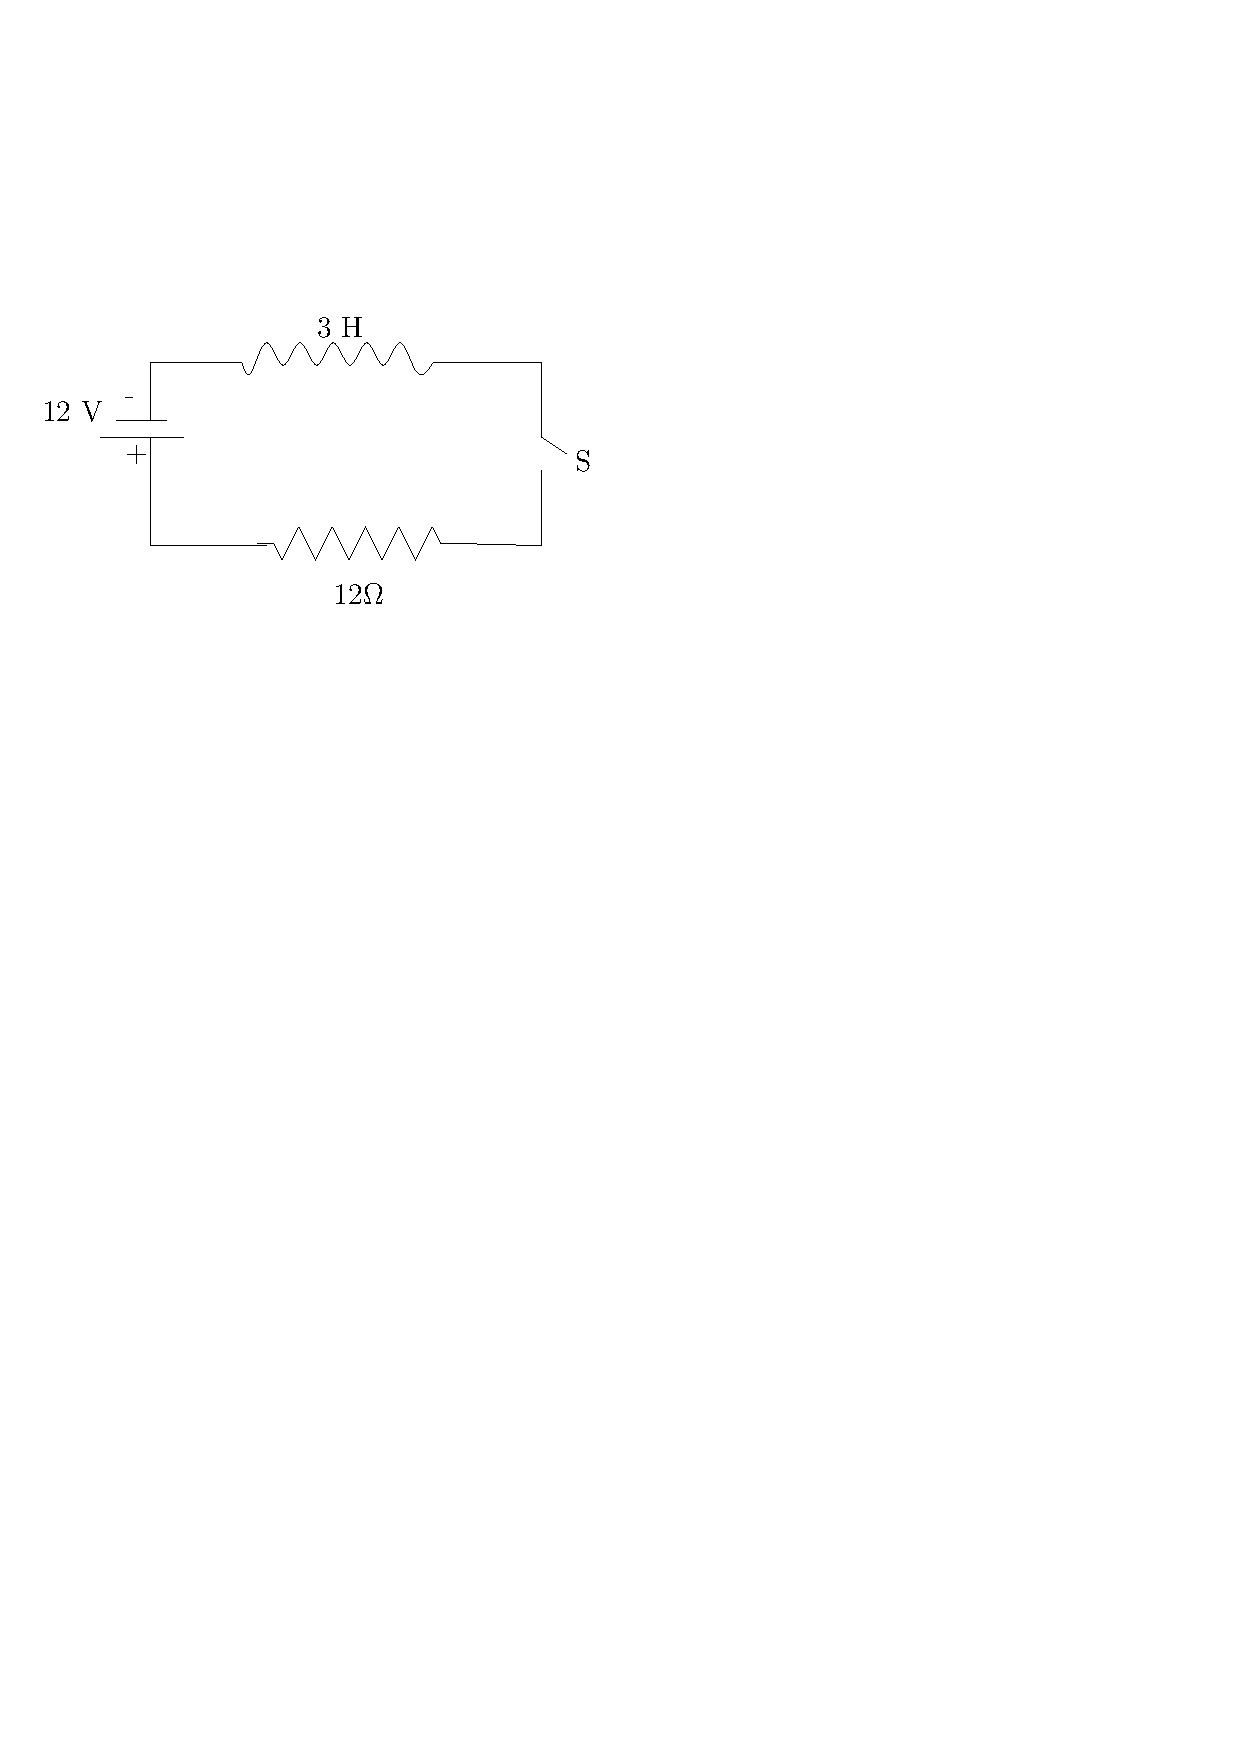
\includegraphics[width=0.4\textwidth]{inductor_circuit.pdf}


\end{document}
